Om de Ritz waarden op te slaan was er een kleine aanpassing nodig in het gegeven algoritme. In elke iteratiestap wordt een kolom van de matrix 'Ritz' aangevuld  met het aantal eigenwaarden op de eerste rij en de berekende eigenwaarden op de rijen hieronder. Met behulp van volgende matlab-code stellen we een figuur op die de re\"ele componenten van de Ritz waarden voorstelt in functie van de iteratiestap n:
\lstinputlisting[
  style      = Matlab-editor,
  basicstyle = \mlttfamily,
]{Arnoldi_oef7.m}

Dit levert het resultaat uit figuur \ref{fig:oef7}. Hierbij stellen de rode waardes rechts de werkelijke eigenvectoren voor en de blauwe de berekende Ritz waarden. Het valt op dat na 100 iteratiestappen en zelfs eerder (<<1000, grootte van de matrix) al een goede benadering van de eigenwaarden bereikt wordt.

\begin{figure}[H]
    \centering
    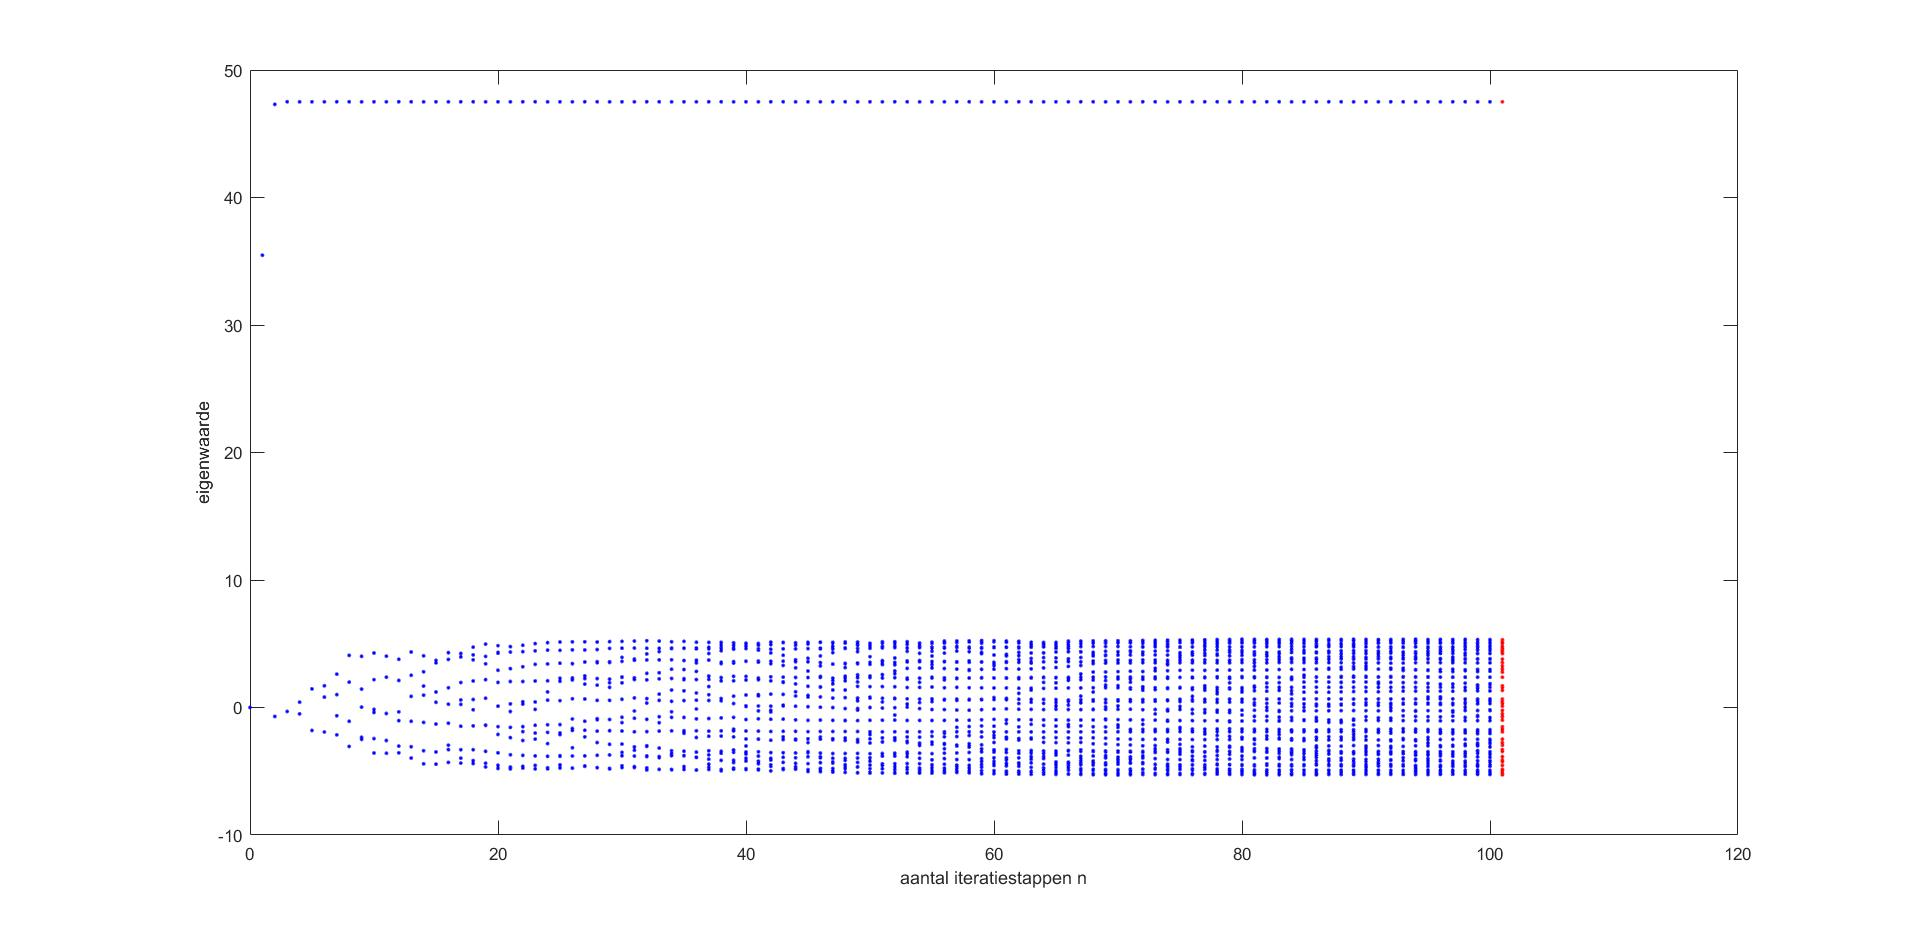
\includegraphics[width=1\textwidth]{oef7.jpg}
    \caption{de Ritz waarden bij verschillende iteratiestappen}
    \label{fig:oef7}
\end{figure}